\subsection{Column correlation}
\label{subsec:pd:columncorrelation}


% ----------------------- paths to graphics ------------------------

\graphicspath{{5_automatic_learning/pattern_detection/images/}}

% ----------------------- contents from here ------------------------
% 

The purpose of the \nameref{subsec:pd:columncorrelation} pattern detector is to find correlations between columns and create mappings that can be used to represent a column as a function of another. The technique we describe is generic and can be applied to any data type. This pattern detector receives an additional parameter \(\mathit{corr\_coef}_{min}\), which indicates the minimum degree of correlation between two columns and is used to filter results in the \textit{evaluation} step. This is a multi-column pattern detector---it needs to analyze multiple columns at the same time.

\textbf{Correlation types.} From a statistical point of view, we can distinguish 3 types of correlations: between continuous, discrete and categorical variables. The first 2 apply to numeric values and can measure numerical similarities (e.g. sales increased as the marketing budget increased). The latter is less restrictive and works with any type of values. Categorical variables contain a finite number of values (e.g. payment method or customer satisfaction levels: low, high, very high, etc.) 
These can be further categorized into ordinal and nominal variables. Ordinal values have a natural ordering (e.g. tiny, small, large, huge) while nominal values have no ordering (e.g. names or colors).

While analyzing the Public BI benchmark we noticed that most correlations are between nominal values. Table~\ref{tab:pd:columncorrelation:nominalexample} shows a representative example from the \textit{CommonGovernment\_1} dataset.

\begin{table}[h]
\centering
\begin{tabular}{@{}ll@{}}
\toprule
short\_name  & ag\_name                                       \\ \midrule
\verb|GSA|   & \verb|GENERAL SERVICES ADMINISTRATION|         \\
\verb|GSA|   & \verb|GENERAL SERVICES ADMINISTRATION|         \\
\verb|HHS|   & \verb|DEPARTMENT OF HEALTH AND HUMAN SERVICES| \\
\verb|TREAS| & \verb|DEPARTMENT OF TREASURY|                  \\
\verb|TREAS| & \verb|DEPARTMENT OF TREASURY|                  \\
\verb|HHS|   & \verb|DEPARTMENT OF HEALTH AND HUMAN SERVICES| \\
\verb|GSA|   & \verb|GENERAL SERVICES ADMINISTRATION|         \\ \bottomrule
\end{tabular}
\caption{CommonGovernment\_1 nominal correlation}
\label{tab:pd:columncorrelation:nominalexample}
\end{table}


The table contains a name and its abbreviation repeated over multiple rows. The 2 columns are perfectly correlated because any value on one of the columns always has the same corresponding value on the other column (e.g. \verb|TREAS| on the \textit{short\_name} column always determines \verb|DEPARTMENT OF TREASURY| on the \textit{ag\_name} column).

Base on this observation, we decided to limit the scope of the \nameref{subsec:pd:columncorrelation} pattern detector to nominal categorical variables and interpret the values on all columns as nominal values. We leave the other correlation types as future work.

\textbf{Correlation coefficient \& mapping.} The \nameref{subsec:pd:columncorrelation} pattern detection process works in 3 phases: 1) compute the correlation coefficient (\(\mathit{corr\_coef}\)) for all pairs of 2 columns (\(c_{source}\), \(c_{target}\)); 2) select the pairs with \(\mathit{corr\_coef}\) higher than \(\mathit{corr\_coef}_{min}\); 3) create the correlation mapping (\(map_{obj}\)) that can be used to determine \(c_{target}\) based on \(c_{source}\).

The measure of association between 2 nominal categorical variables can be determined through existing statistical methods like Cramer's V \cite{cramir1946mathematical} or the Uncertainty coefficient Theil's U \cite{press1992theilsu}. Both methods are suitable for finding correlations between columns, but they only provide the measure of how well the columns are correlated as a number between 0 and 1---the correlation coefficient \(\mathit{corr\_coef}\). We still need the correlation mapping to be able to represent one column as a function of another.

We define the correlation mapping \(map_{obj}\) between 2 columns \(c_{source}\) and \(c_{target}\) as a dictionary with (\(v_{source}\), \(v_{target}\)) key-value pairs, where \(v_{source}\) are values from \(c_{source}\) and \(v_{target}\) are values from \(c_{target}\). Formally, the mapping is a total function \(f \colon S \to T\), where an element from T can be mapped to 0, 1 or multiple elements in S, as depicted in Figure~\ref{fig:pd:columncorrelation:totalfunction}.

\begin{figure}[h]
  \centering
  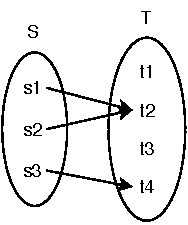
\includegraphics[width={0.23\linewidth}]{total_function_2.pdf}
  \caption{Mapping function}
  \label{fig:pd:columncorrelation:totalfunction}
\end{figure}

The process of creating the mapping between 2 columns \(c_{source}\) and \(c_{target}\) is depicted in Figure~\ref{fig:pd:columncorrelation:mapping}.

\begin{figure}[h]
  \centering
  \begin{subfigure}[t]{0.22\linewidth}
    \centering
    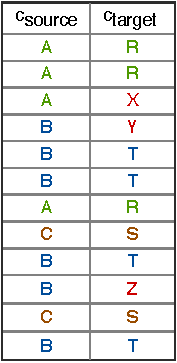
\includegraphics[width=1\linewidth]{mapping-corr-step_1_1.pdf}
    \caption[b]{Data values}
    \label{fig:pd:columncorrelation:mapping:step1}
  \end{subfigure}
  \hspace{3em}
  \begin{subfigure}[t]{0.23\linewidth}
    \centering
    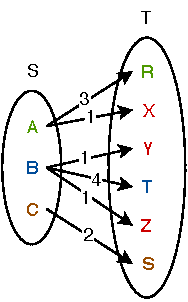
\includegraphics[width=1\linewidth]{mapping-corr-step_2_1.pdf}
    \caption[b]{Step-1}
    \label{fig:pd:columncorrelation:mapping:step2}
  \end{subfigure}
  \hspace{3em}
  \begin{subfigure}[t]{0.23\linewidth}
    \centering
    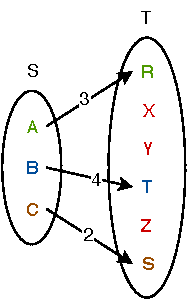
\includegraphics[width=1\linewidth]{mapping-corr-step_3_1.pdf}
    \caption[b]{Step-2}
    \label{fig:pd:columncorrelation:mapping:step3}
  \end{subfigure}
  \caption{Column correlation mapping}
  \label{fig:pd:columncorrelation:mapping}
\end{figure}

The correlation mapping is built in 2 steps. Step-1: for every unique value in \(c_{source}\) build the histogram of values in \(c_{target}\) it is associated with. In the example in Figure~\ref{fig:pd:columncorrelation:mapping}, \verb|B| is associated with \verb|T| 4 times and with \verb|Y| and \verb|Z| one time. Step-2: for every unique value in \(c_{source}\) select the value in \(c_{target}\) it is associated with the most (i.e. the one with the highest number of occurrences). In the example, \verb|R| is the most common value for \verb|A|, \verb|T| is the most common value for \verb|B| and \verb|S| is the only value associated with \verb|C|. These selected pairs of values form the correlation mapping \(map_{obj}\).

We consider exceptions all the values from \(c_{target}\) that are not present in \(map_{obj}\). The \(exception\_ratio\) is given by the total number of values on \(c_{target}\) that do not respect the correlation mapping.

\begin{figure}[h]
\centering
\makebox[\textwidth][c]{
    \includesvg[width={1.05\linewidth}]{merged-s_1_l_0-coefs.svg}
}
\caption{Correlation coefficients comparison (\textit{YaleLanguages\_1})}
\label{fig:pd:columncorrelation:corrcoefs}
\end{figure}

We observe that two columns that have \(exception\_ratio = 0\) are perfectly correlated (i.e. all values in \(c_{target}\) can be determined from \(c_{source}\)). Conversely, two columns with \(exception\_ratio = 1\) are completely uncorrelated. We can define, then, an alternative correlation coefficient: 
\(\mathit{corr\_coef} = 1 - exception\_ratio\). We compared it with Cramer's V and Theil's U by computing the correlation coefficient for tables in the Public BI benchmark. Figure~\ref{fig:pd:columncorrelation:corrcoefs} shows the coefficients resulted from the compression learning process on the \textit{YaleLanguages\_1} table. Each image shows the correlation coefficients between every pair of columns (note that these are not logical columns, but intermediate columns resulted from the learning process---more details will follow in chapters \ref{ch:automaticlearning} and \ref{ch:evaluation}). Bright colors indicate high coefficients and dark colors low coefficients. We notice how all three images have a similar shape/pattern: the white rectangles from the first image are also visible in the other two and their internal shape is almost identical in the last two images. Our approach gives higher overall coefficients, but it is consistent with the other two approaches when it comes to identifying near-perfect correlations: all pairs of columns with correlation coefficient \(\approx{1.0}\) are also identified by Cramer's V and Theil's U. Based on these results, we decided to use our own version of computing the correlation coefficient (\(1 - exception\_ratio\)) instead of the other approaches for the following reason: for our purpose, correlation is only useful if we can represent columns as functions of other columns through correlation mappings. These mappings will determine the exceptions, which will, in turn, determine the size of the physical data and implicitly the compression ratio. Therefore, the correlation coefficient, as we defined it above, gives the most accurate estimation of how suitable two columns are for correlation representation. In this context, Cramer's V and Theil's U do not bring any advantage over our approach and even if we were to use them instead, we would still need to compute the correlation mapping. Moreover, we are only interested in highly correlated columns which are similarly identified by all approaches (more details about the selection of column pairs based on their correlation coefficient are discussed in \ref{subsubsec:ps:correlation}~\nameref{subsubsec:ps:correlation} and \ref{sec:eval:expsetup}~\nameref{sec:eval:expsetup}).

Coming back to the pattern detection process, the histograms---necessary for creating the correlation mappings---are built in the \textit{scanning} phase and the correlation coefficients and mappings are computed in the \textit{evaluation} phase. The compression and decompression metadata resulted from this process is the correlation map \(map_{obj}\). The pattern detector outputs all (\(c_{source}, c_{target}\)) pairs with \(\mathit{corr\_coef} > \mathit{corr\_coef}_{min}\), leaving the task of choosing between the results to the learning algorithm. The \textit{evaluation result} is composed of the \textit{coverage} and \textit{row\_mask}---as defined in \ref{subsec:genericpd}~\nameref{subsec:genericpd}---and the correlation coefficient.

The \textit{expression nodes} for the \nameref{subsec:pd:columncorrelation} pattern are illustrated in Figure~\ref{fig:pd:columncorrelation:exprnode}.

\begin{figure}[h]
  \centering
  \begin{subfigure}[t]{0.45\linewidth}
    \centering
    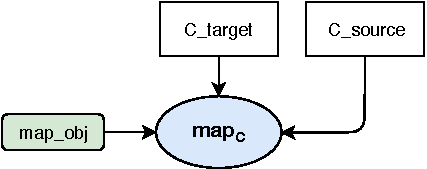
\includegraphics[width=1\linewidth]{expression_node-corr-compression_3.pdf}
    \caption[b]{compression}
    \label{fig:pd:columncorrelation:exprnode:compression}
  \end{subfigure}
  \hspace{3em}
  \begin{subfigure}[t]{0.30\linewidth}
    \centering
    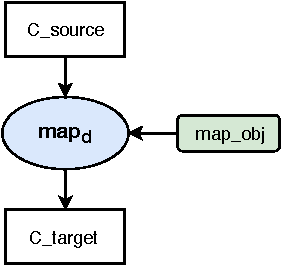
\includegraphics[width=1\linewidth]{expression_node-corr-decompression_3.pdf}
    \caption[b]{decompression}
    \label{fig:pd:columncorrelation:exprnode:decompression}
  \end{subfigure}
  \caption{Column correlation expression nodes}
  \label{fig:pd:columncorrelation:exprnode}
\end{figure}

The \textit{compression node} takes as input the target column (\(c_{target}\)), the source column (\(c_{source}\)) and the metadata (\(map_{obj}\)). It does not generate any output column. The \textit{decompression node} takes as input \(c_{source}\) and \(map_{obj}\) and reconstructs \(c_{target}\) based on the mapping.

The compression operator \(map_{c}\) takes as input a target value (\(v_{target}\)), a source value (\(v_{source}\)) and the metadata (\(map_{obj}\)) and checks whether the key-value pair (\(v_{source}\), \(v_{target}\)) is present in \(map_{obj}\). If true, then it does nothing---\(v_{target}\) can be reconstructed based on \(v_{source}\). Otherwise, it raises an \textit{OperatorException} indicating that \(v_{target}\) cannot be retrieved from the mapping and needs to be stored in the exception column. The decompression operator \(map_{d}\) takes as input \(v_{source}\) and \(map_{obj}\) and returns the value from \(map_{obj}\) associated to \(v_{source}\): \(map_{obj}[v_{source}] = v_{target}\).

The benefit of the \nameref{subsec:pd:columncorrelation} compression scheme is clear: we avoid storing a column by representing it as a function of another column. However, this comes at the cost of storing the mapping between the 2 columns. Thus, it is only worth using this method when the mapping is small. The mapping size is dependent on the cardinality of the sets of values in the 2 columns. This is similar to \nameref{subsec:pd:dict} encoding and therefore we can state that \nameref{subsec:pd:columncorrelation} is effective only when both source and target columns are dictionary compressible.  With this new constraint, we can limit the scope of the \nameref{subsec:pd:columncorrelation} pattern detector to output columns of \textit{whitebox} \nameref{subsec:pd:dict} nodes, leading to the following benefits: 1) reduced detection time---less column pairs that need to be checked; 2) reduced mapping size---dictionary ids instead of string values. Due to the generic nature of \textit{whitebox} compression, this constraint can be implicitly satisfied by just adding a rule to the \textit{select\_column} method of the \nameref{subsec:pd:columncorrelation} pattern detector and letting the learning algorithm perform the recursive compression.


\iffalse
- have a somewhat similar shape
- our approach seems to give higher overall coefs, but both give perfect correlation score (1.0) to the same columns (both make the distinction between perfectly correlated columns and the others)
- we are only interested in close to perfect correlations, therefore...
- for our purpose correlation is only useful if we can represent a column as a mapping of another
- the exceptions will be given solely by the mapping; the correlation coef is the inverse of the exceptions
- the corr coef, mapping and expcetion rate are strictly dependable on each other. therefor our compression ratio will depend on them;
for this reason we chose to use our correlation coef instead of CV or TU; they do not bring any addtional value
- regardless of the differecens between the 3, we will use...
\fi

% We analyzed the results and concluded that all three methods are similar and correctly identify correlations between nominal columns. The advantage of our approach is that it also gives the correlation mapping---which we are interested in---without any time complexity overhead: \(\mathcal{O}(n)\), where \(n\) is the total number of values in the sample. For this reason, we decided to use it in our implementation instead of Cramer's V or Theil's U.

% ---------------------------------------------------------------------------
% ----------------------- end of thesis sub-document ------------------------
% ---------------------------------------------------------------------------
